\subsection{Business}
Il progetto Scalavelli vuole ricreare l’esperienza del celebre gioco di carte Machiavelli (Ramino Machiavellico) in modalità multiplayer, tra giocatori differenti collocati sulla stessa macchina o nella stessa LAN. Ogni giocatore deve potersi identificare con un proprio username e connettersi ad una lobby.
Essa deve poter contenere da 2 a 6 giocatori.
Raggiunto il numero necessario di essi si potrà partecipare ad una partita.
Vi è anche la possibilità di scegliere di giocare specificatamente con i propri amici inserendo il codice identificativo per una partita privata.

\subsection{Utente}
L’utente medio utilizzatore potrà interagire solamente con il client (come descritto in seguito).
Le operazioni in fase di creazione della partita sono:
\begin{itemize}
    \item Specificare il proprio username (per potersi registrare nel server) e il numero di giocatori di una partita pubblica;
    \item Specificare il proprio username e il codice di una partita privata che gli è stato inviato;
    \item Specificare il proprio username, il numero di giocatori e generare un codice per una partita privata;
    \item Inserire o creare una lobby privata;
    \item Connettersi ad una lobby e attendere il raggiungimento del numero di giocatori.
\end{itemize}
Dopo aver generato una partita ed esservi entrato, in una nuova schermata il giocatore potrà:
\begin{itemize}
    \item Vedere sullo schermo le combinazioni che ci sono attualmente sul tavolo da gioco, le carte che ha in mano, il nome degli altri giocatori e il numero di carte nelle loro mani;
    \item Solamente nel proprio turno, eseguire le seguenti azioni:
    \begin{itemize}
        \item Giocare una combinazione: si possono mettere sul tavolo da giocare una sequenza di carte che compongono una combinazione tra un tris, un poker oppure una scala.
        Se la combinazione è valida, allora vengono tolte le carte che si vuole giocare dalla mano e vengono messe sul tavolo;
        \item Aggiungere carte ad una combinazione sul tavolo già esistente: si possono scegliere delle carte dalla propria mano, che non necessariamente compongono una combinazione valida e mettere assieme alle carte che compongono un’altra combinazione, a patto che venga sempre rispettata la validità della combinazione;
        \item Prendere delle carte dal tavolo: si possono scegliere delle carte che appartengono ad una combinazione presente sul tavolo da gioco e metterle nella propria mano.
        \item Passare il turno al giocatore successivo: dopo che viene eseguita questa azione, il turno viene passato al giocatore successivo.
        Il giocatore che ha eseguito questa azione non ne può effettuare nessun’altra fino a che non riprende il proprio turno dall’azione del giocatore precedente nell’ordine.
        Nel caso in cui il giocatore di turno:
        \begin{itemize}
            \item non avesse eseguito nessuna mossa;
            \item avesse in mano delle carte che ha preso dal tavolo da gioco senza averle rigiocate;
            \item se non si trovasse con meno carte in mano rispetto a quando ha iniziato il turno;
            \item se scade il tempo a disposizione;
        \end{itemize}
        allora è costretto a pescare una carta dal mazzo principale.
    \end{itemize}
\end{itemize}

\subsection{Funzionali}
\begin{center}
    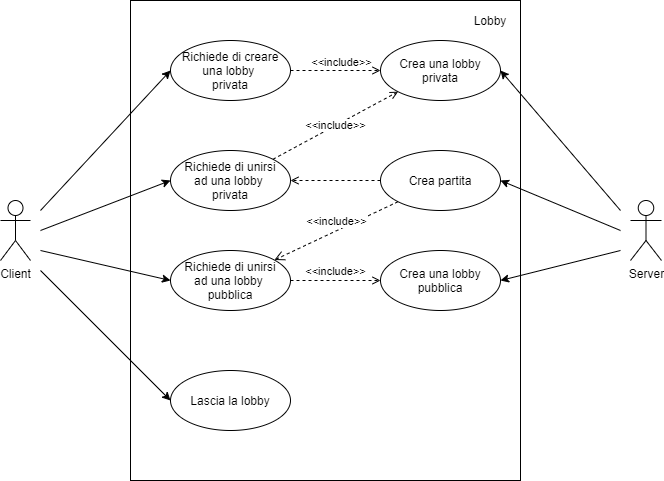
\includegraphics[scale=0.4]{casiDUso_Lobby}
\end{center}
\subsubsection{Connessione al server e creazione della lobby}
Il sistema dovrà:
\begin{itemize}
    \item Permettere al client di connettersi a internet;
    \item Una volta connessi al server permettersi di unirsi ad una lobby attraverso il proprio username;
    \item Assicurarsi che il server mantenga sempre attiva la connessione con il client, per poter inviare e ricevere messaggi inerenti alla partita;
    \item Assicurarsi che qualora venga raggiunto il numero di giocatori necessario, il server dovrà subito far partire la partita tra i giocatori;
    \item Nel caso in cui un giocatore venga disconnesso dalla partita, sia una disconnessione volontaria o un problema dell’infrastruttura di rete, terminare la partita per tutti, venendo visto come un abbandono;
    \item Al termine di una partita permetterne di iniziarne una nuova.
\end{itemize}
\begin{center}
    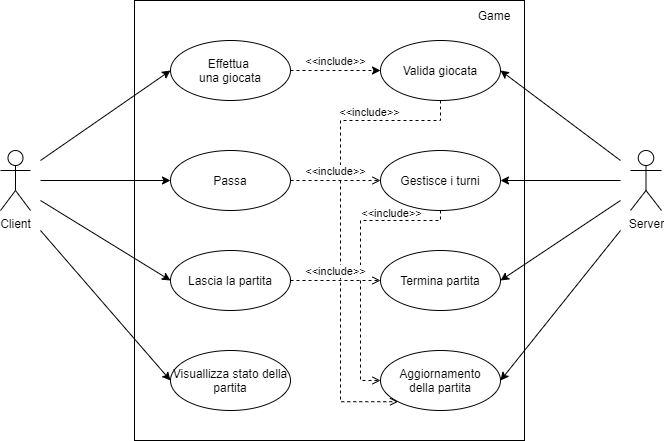
\includegraphics[scale=0.4]{casiDUso_Game}
\end{center}
\subsubsection{Gioco}
All’inizio della partita vengono mischiati due mazzi da 52 carte ognuno e distribuite 13 carte ad ogni giocatore.
Nel proprio turno si ha un tempo massimo di 2 minuti per svolgere le proprie mosse.
Una volta scaduto, tutte le mosse effettuate vengono annullate, si pesca una carta e si passa il turno al giocatore successivo.
In ogni momento devono sempre essere visibili:
\begin{itemize}
    \item le proprie carte in mano;
    \item il tavolo da gioco con le varie combinazioni;
    \item gli altri giocatori, con i loro nomi e il numero di carte nelle loro mani.
\end{itemize}

\subsection{Non Funzionali}

\subsubsection{Scalabilità}
Il server deve essere in grado di supportare un numero indefinito di utenti nell’insieme di tutte le partite.
Nel caso in cui non ci siano abbastanza giocatori in coda per iniziare una partita, allora devono essere lasciati in attesa dell’arrivo di altri giocatori che vogliano giocare anche loro.
Il sistema non consente l’accesso ad altri utenti per una partita specifica quando questa ha raggiunto il numero di partecipanti richiesto.

\subsubsection{Modularità}
Il progetto è stato pensato in modo tale da dover effettuare meno modifiche possibili al client nel caso in cui debba essere cambiato il server e viceversa.
Nello specifico: se il server deve subire un aggiornamento, esso dovrebbe essere spento e poi riacceso.
Gli utenti finali non devono eseguire nessuna operazione sui loro client, o almeno l’aggiornamento deve essere mantenuto il più piccolo possibile.
Viceversa, nel caso di aggiornamento dei client, non dovrebbe essere necessario né riavviare il server, né aggiornare nessuna sua parte.
Tutto il software deve riuscire a funzionare anche cambiando l’implementazione interna del modulo del “core” (regole e logica di gioco) a patto di non impattare sull’interfaccia dello stesso.

\subsubsection{Usabilità}
Il sistema deve fornire agli utenti un'interfaccia chiara, semplice, ben organizzata in modo da poter utilizzare al meglio tutte le sue funzionalità messe a disposizione e visualizzate.

\subsubsection{Reattività}
Il sistema deve poter consentire di giocare una partita senza ritardi e/o blocchi temporali dati dall’esecuzione degli algoritmi di validazione e controllo e dai protocolli di comunicazione.

\subsubsection{Sicurezza}
Il sistema deve aver sempre la possibilità di controllare lo stato attuale del gioco in modo da impedire che alcuni giocatori possano iniettarne uno non veritiero nella partita attuale.
Per questo ad ogni fine turno deve essere validato da parte del server in modo che un client malevolo non possa rovinare l’esperienza di gioco agli altri giocatori.

\subsection{Implementativi}
Di seguito vengono descritti i vincoli che abbiamo cercato di rispettare per l’intero sviluppo del progetto:
\begin{itemize}
    \item Mantenere un approccio il più funzionale possibile;
    \item Mantenere, in tutti i casi in cui era possibile, una stato immutabile nei vari componenti del sistema.
\end{itemize}
Principali tecnologie e modelli utilizzati sono:
\begin{itemize}
    \item Scala: Il sistema deve essere prevalentemente sviluppato in scala.
    \item ScalaFX: Il sistema deve disporre di un’interfaccia grafica per poter interagire con il gioco e il server.
    \item Prolog: Utilizzo del prolog per implementare l’ordinamento delle carte (per seme, valore e colore), le entità del gioco e la validazione della correttezza delle combinazioni di carte.
    \item Akka: Utilizzo di varie componenti per implementare un server e un client che comunichino, secondo il paradigma di programmazione ad attori, per mezzo di messaggi asincroni.
    \item TDD (Test Driven Development): Ci siamo ispirati a questa tecnica di sviluppo per scrivere un codice più efficiente, efficace e il più possibile esente da problemi.
\end{itemize}
\newpage